\newcommand{\nom}{Porte conteneur}
\newcommand{\sequence}{03}
\newcommand{\num}{04}
\newcommand{\type}{TD}
\newcommand{\descrip}{Résolution d'un problème en utilisant des méthodes algorithmiques}
\newcommand{\competences}{Alt-C3: Concevoir un algorithme répondant à un problème précisément posé}
\documentclass[10pt,a4paper]{article}
  \usepackage[french]{babel}
  \usepackage[utf8]{inputenc}
  \usepackage[T1]{fontenc}
  \usepackage{xcolor}
  \usepackage[]{graphicx}
  \usepackage{makeidx}
  \usepackage{textcomp}
  \usepackage{amsmath}
  \usepackage{amssymb}
  \usepackage{stmaryrd}
  \usepackage{fancyhdr}
  \usepackage{lettrine}
  \usepackage{calc}
  \usepackage{boxedminipage}
  \usepackage[french,onelanguage, boxruled,linesnumbered]{algorithm2e}
  \usepackage[colorlinks=false,pdftex]{hyperref}
  \usepackage{minted}
  \usepackage{url}
  \usepackage[locale=FR]{siunitx}
  \usepackage{multicol}
  \usepackage{tikz}
  \makeindex

  %\graphicspath{{../Images/}}

%  \renewcommand\listingscaption{Programme}

  %\renewcommand{\thechapter}{\Alph{chapter}}
  \renewcommand{\thesection}{\Roman{section}}
  %\newcommand{\inter}{\vspace{0.5cm}%
  %\noindent }
  %\newcommand{\unite}{\ \textrm}
  \newcommand{\ud}{\mathrm{d}}
  \newcommand{\vect}{\overrightarrow}
  %\newcommand{\ch}{\mathrm{ch}} % cosinus hyperbolique
  %\newcommand{\sh}{\mathrm{sh}} % sinus hyperbolique

  \textwidth 160mm
  \textheight 250mm
  \hoffset=-1.70cm
  \voffset=-1.5cm
  \parindent=0cm

  \pagestyle{fancy}
  \fancyhead[L]{\bfseries {\large PTSI -- Dorian}}
  \fancyhead[C]{\bfseries{{\type} \no \numero}}
  \fancyhead[R]{\bfseries{\large Informatique}}
  \fancyfoot[C]{\thepage}
  \fancyfoot[L]{\footnotesize R. Costadoat, C. Darreye}
  \fancyfoot[R]{\small \today}
  
  \definecolor{bg}{rgb}{0.9,0.9,0.9}
  
  
  % macro Juliette
  
\usepackage{comment}   
\usepackage{amsthm}  
\theoremstyle{definition}
\newtheorem{exercice}{Exercice}
\newtheorem*{rappel}{Rappel}
\newtheorem*{remark}{Remarque}
\newtheorem*{defn}{Définition}
\newtheorem*{ppe}{Propriété}
\newtheorem{solution}{Solution}

\newcounter{num_quest} \setcounter{num_quest}{0}
\newcounter{num_rep} \setcounter{num_rep}{0}
\newcounter{num_cor} \setcounter{num_cor}{0}

\newcommand{\question}[1]{\refstepcounter{num_quest}\par
~\ \\ \parbox[t][][t]{0.15\linewidth}{\textbf{Question \arabic{num_quest}}}\parbox[t][][t]{0.85\linewidth}{#1\label{q\the\value{num_quest}}}\par
~\ \\}

\newcommand{\reponse}[4][1]
{\noindent
\rule{\linewidth}{.5pt}\\
\textbf{Question\ifthenelse{#1>1}{s}{} \multido{}{#1}{%
\refstepcounter{num_rep}\ref{q\the\value{num_rep}} }:} ~\ \\
\ifdef{\public}{#3 ~\ \\ \feuilleDR{#2}}{#4}
}

\newcommand{\cor}
{\refstepcounter{num_cor}
\noindent
\rule{\linewidth}{.5pt}
\textbf{Question \arabic{num_cor}:} \\
}

%%\usepackage[a4paper]{geometry}
%\geometry{margin={1cm,1.2cm}}
%\usepackage[francais]{babel}
%\usepackage{nopageno} %pas de numérotation de page
%\pagestyle{plain} %numérotation en bas de page, pas d'entête
%\usepackage{hyperref}
%\usepackage[latin1]{inputenc}

%%%%%%%%%%%%%%%%%%%%%%%%%%%%%%%%%%%%%%%%%%%%%%%%%%%%%%%%%%%%%%%%%%%%%%%%%%%%%%%%%%%%%

\usepackage{amsthm}
\usepackage{amscd}
%\usepackage{mathrsfs}
%\usepackage{amsfonts}
%\usepackage[T1]{fontenc}
%\usepackage{theorem}
\usepackage{lscape}
\usepackage{variations}  % pour faire des tableaux de variations
\usepackage{dsfont}
\usepackage{fancyvrb} % pour mettre Verbatim dans une box

% Pour les figures
\usepackage{subfig}
%\usepackage{calc} % Pour pouvoir donner des formules dans les d�finitions de longueur
%\usepackage{graphicx} % Pour inclure des graphiques 
% Attention : pour inclure des .jpg comme dans l'exemple (ou des .png ou .pdf)
% il faut compiler directement en pdf (commande pdflatex).
% Pour inclure des .eps, il faut compiler avec latex + dvips + ps2pdf.
\usepackage{psfrag}
%\usepackage{color}

%%%%%%%%%%%%%%%%%%%%%%%%%%%%%%%%%%%%%%%%%%%%%%%%%%%%%%%%%%%%%%%%%%%%%%%%%%%%%%%%%%%%%

\theoremstyle{definition}
\newtheorem*{thm}{Théorème}
%\theorembodyfont{\rmfamily}
\newtheorem*{defn}{Définition}
\newtheorem{exercice}{Exercice}
\newtheorem*{problem}{Problème}
\newtheorem*{prop}{Proposition}
\newtheorem*{corollaire}{Corollaire}
\newtheorem*{lemme}{Lemme}
\newtheorem*{remark}{Remarque}
\newtheorem*{notation}{Notation}
\newtheorem*{ex}{Exemple}
\newtheorem*{ppe}{Propriété}
\newtheorem*{meth}{Méthode}
\newtheorem*{rappel}{Rappel}
\newtheorem*{voca}{Vocabulaire}
\setlength{\columnseprule}{0.5pt}


%%%%%%%%%%%%%%%%%%%%%%%%%%%%%%%%%%%%%%%%%%%%%%%%%%%%%%%%%%%%%%%%%%%%%%%%%%%%%%%%%%%%%

\newcommand{\bi}{\bigskip}
\newcommand{\dsp}{\displaystyle}
\newcommand{\noi}{\noindent}
\newcommand{\ov}{\overline}
\newcommand{\dsum}{\displaystyle \sum}
\newcommand{\dprod}{\displaystyle \prod}
\newcommand{\dint}{\displaystyle \int}
\newcommand{\dlim}{\displaystyle \lim}

%%%%%%%%%%%%%%%%%%%%%%%%%%%%%%%%%%%%%%%%%%%%%%%%%%%%%%%%%%%%%%%%%%%%%%%%%%%%%%%%%%%%%


%\newcommand{\pgcd}{\mathrm{pgcd}} % pgcd
%\providecommand{\norm}[1]{\lVert#1\rVert} % norme
%\DeclareMathOperator{\Tan}{Tan}  % espace tangent


\newcommand{\N}{\mathbb{N}}
\newcommand{\Z}{\mathbb{Z}}
\newcommand{\Q}{\mathbb{Q}}
\newcommand{\R}{\mathbb{R}}
\newcommand{\C}{\mathbb{C}}
\newcommand{\K}{\mathbb{K}}
\newcommand{\U}{\mathbb{U}}
\newcommand{\Tr}{\text{Tr}\,}
\newcommand{\pg}{\geqslant}
\newcommand{\pp}{\leqslant}
\newcommand{\bul}{\item[$\bullet$]}
\newcommand{\card}{\text{Card}}
\newcommand{\re}{\text{Re}\;}
\newcommand{\im}{\text{Im}\;}
\newcommand{\Ker}{\text{Ker}\;}
\newcommand{\Vect}{\text{Vect}\;}
\newcommand{\rg}{\text{rg}\;}
\newcommand{\TT}{{}^t\!}
%\newcommand{\sh}{\text{sh}}
%\newcommand{\ch}{\text{ch}}
\newcommand{\Mat}{\text{Mat}}
\usepackage{textcomp}



%%%%%%%%%%%%%%%%%%%%%%%%%%%%%%%%%%%%%%%%%%%%%%%%%%%%%%%%%%%%%%%%%%%%%%%%%%%%%%%%%%%%%%%%%%%%%%%%%%%%%%%%%%%%%%%%%%%%%%%%%%%




\begin{document}

\begin{center}
{\Large\bf TP \no {\numero} -- \descrip}
\end{center}

\begin{small}\textit{D'après un TP de E. Bougnol, J.J. Fleck, M. Heckmann et M. Kostyra, Lycée Kléber.}\end{small}
 
\section*{Contexte général}

En astro-informatique, la méthode d’Euler est souvent utilisée pour intégrer numériquement les équations du mouvement des objets en interaction gravitationnelle. On va étudier ici le cas particulier d’une masse $m$ supposée ponctuelle soumise à l’attraction gravitationnelle d’une masse $M$ bien plus importante placée au centre $O$ du repère et fixe dans le référentiel d'étude. Les équations du mouvement s’écrivent alors de manière vectorielle :


\begin{multicols}{2}
En coordonnées cartésiennes :
\begin{displaymath}
\left\{ \begin{array}{lll}
\ddot{x} & = & \displaystyle - \frac{G\,M}{\left(x^2+y^2\right)^{\frac{3}{2}}}\,x  \\
\ddot{y} & = & \displaystyle - \frac{G\,M}{\left(x^2+y^2\right)^{\frac{3}{2}}}\,y 
\end{array} \right.
\end{displaymath}

$$E = \frac{1}{2}\,m\,(\dot{x}^2+\dot{y}^2)- \frac{G\,M\,m}{\sqrt{x^2+y^2}}$$

    \columnbreak
En coordonnées polaires :
\begin{displaymath}
\left\{ \begin{array}{lll}
\ddot{r}-r\,\dot{\theta}^2 & = & \displaystyle - \frac{G\,M}{r^2} \\
2\dot{r}\dot{\theta}+r\ddot{\theta} & = & 0 
\end{array} \right.
\end{displaymath}

$$E = \frac{1}{2}\,m\,(\dot{r}^2+(r\,\dot{\theta})^2)- \frac{G\,M\,m}{r}$$

\end{multicols}

En bons astro-informaticiens, nous prendrons les termes constants $G$, $M$ et $m$ tous égaux à 1 unité SI, de sorte que les équations soient vraiment simples à écrire.

\vspace{1cm}

\begin{boxedminipage}{\textwidth}

\begin{multicols}{2}
En coordonnées cartésiennes :
\begin{displaymath}
\left\{ \begin{array}{lll}
\ddot{x} & = & \displaystyle - \frac{1}{\left(x^2+y^2\right)^{\frac{3}{2}}}\,x  \\
\ddot{y} & = & \displaystyle - \frac{1}{\left(x^2+y^2\right)^{\frac{3}{2}}}\,y 
\end{array} \right.
\end{displaymath}

$$E = \frac{1}{2}\,(\dot{x}^2+\dot{y}^2)- \frac{1}{\sqrt{x^2+y^2}}$$

    \columnbreak

En coordonnées polaires :
\begin{displaymath}
\left\{ \begin{array}{lll}
\ddot{r} & = & \displaystyle - \frac{1}{r^2} + r\,\dot{\theta}^2 \\
\ddot{\theta} & = & -\frac{2}{r}\,\dot{r}\dot{\theta} 
\end{array} \right.
\end{displaymath}

$$E = \frac{1}{2}\,(\dot{r}^2+(r\,\dot{\theta})^2)- \frac{1}{r}$$

\end{multicols}
\vspace{0.25cm}
\end{boxedminipage}

\vspace{1cm}

Un des buts du TP est de constater que, pour ce problème particulier et en utilisant la méthode d'Euler classique, les calculs en coordonnées cartésiennes sont en général moins précis que les calculs en coordonnées polaires.

\section{Intégration par la méthode d'Euler}

On va intégrer les deux systèmes d’équations par la méthode d’Euler pour vérifier si le choix du repère influence la précision des calculs. On évaluera aussi l’influence du pas de temps en unités arbitraires (par exemples : \verb|dt=1e-2| ou \verb|1e-3| ou \verb|1e-4|) sur les résultats d’intégration. On limitera le nombre total de points à afficher à 1000 en ne stockant que des échantillons prélevés à intervalle régulier entre \verb|0| et \verb|tfinal|. 

Outre l'aspect visuel qualitatif des trajectoires obtenues, un critère quantitatif de la précision de nos calculs sera la conservation de l'énergie calculée. On pourra notamment déterminer la fluctuation maximale $100\,\frac{E_{max}-E_{min}}{|E_{min}|}$ de l'énergie calculée entre l'instant initial et la fin de l'intégration par la méthode d'Euler. Pour cela, on calculera également à chaque pas de sortie l'énergie. 

\newpage

L’algorithme à considérer est le suivant :
 \begin{itemize}
\item Initialisation des valeurs de position et vitesse. Les valeurs \verb|x0=1, y0=0, vx0=0, vy0=1| conduisant à une trajectoire circulaire (si \verb|G=M=m=1|), il est conseillé de commencer avec ce type de conditions initiales pour vérifier que l'intégration fonctionne correctement. De même, pour débuter tout en limitant le temps de calcul, on prendra \verb|tfinal=100| et \verb|dt=1e-2|.
\item On boucle le calcul pour aller de l'instant initial à l'instant final. À chaque étape , on met à jour l'accélération, puis la position, puis la vitesse\footnote{On prend soin de respecter cet ordre. En effet, $a(t)$ dépend de $x(t)$ et $y(t)$, il faut donc mettre à jour l'accélération avant d'avoir mis à jour la position. De même, $x(t+dt) = x(t) + vx(t) dt$ donc il faut mettre à jour la position avant d'avoir mis à jour la vitesse.}, puis le temps (\verb|x = x + vx*dt|, \verb|y = y + vy*dt|, \verb|vx = vx + ax*dt|, \verb|vy = vy + ay*dt|,  \verb|t= t + dt|).
 \item Si \verb|t| correspond à un des millièmes du temps final, on calcule l'énergie et on stocke les valeurs de positions, d'énergie et de temps dans des listes. 
 \item Une fois l'intégration terminée on affiche la fluctuation en énergie pour chacune des méthodes et on trace les courbes. 
\end{itemize}

Il va donc falloir écrire deux fonctions : \verb|euler_cartesien(x0,vy0,dt,tfinal)| et\\ \verb|euler_polaire(x0,vy0,dt,tfinal)| qui acceptent toutes deux en entrée les valeurs de position et de vitesse initiales en coordonnées cartésiennes, la valeur du pas de temps \verb|dt| et le temps final \verb|tfinal|. 

Ces deux fonctions doivent renvoyer quatre listes \verb|x,y,t,E| comprenant respectivement les coordonnées cartésiennes $x$ et $y$, ainsi que les temps $t$ et énergies $E$ pour chacun des 1000 points que l’on utilisera pour l’affichage final. 

Pour l'intégration en coordonnées polaires, on rappelle les formules utiles permettant le passage initial de cartésiennes à polaires dans ces conditions simples ($y_0 = 0$ et $v_{x0} = 0$)\footnote{Attention, si $y_0 \neq 0$ ou $v_{x0} \neq 0$, les relations de passage sont beaucoup plus compliquées. Voir Annexes.} :

\begin{center}$r_0 = x_0$, $\theta_0=0$, $\dot{r}_0 = 0$ et $\dot{\theta}_0 = \frac{v_{y0}}{r_0}$\end{center}

et, réciproquement, à tout instant pour renvoi des listes demandées en fin de procédure :

\begin{center}$x=r\,\cos(\theta)$ et $y=r\,\sin(\theta)$\end{center}

Une fois l'algorithme implanté en python, modifier les conditions initiales ($x_0$ et $v_{y0}$), $dt$, $t_f$ pour voir leurs effets sur la précision de calcul et sur la trajectoire calculée.

\vspace{1cm}

\begin{figure}[htp]
 \centering
 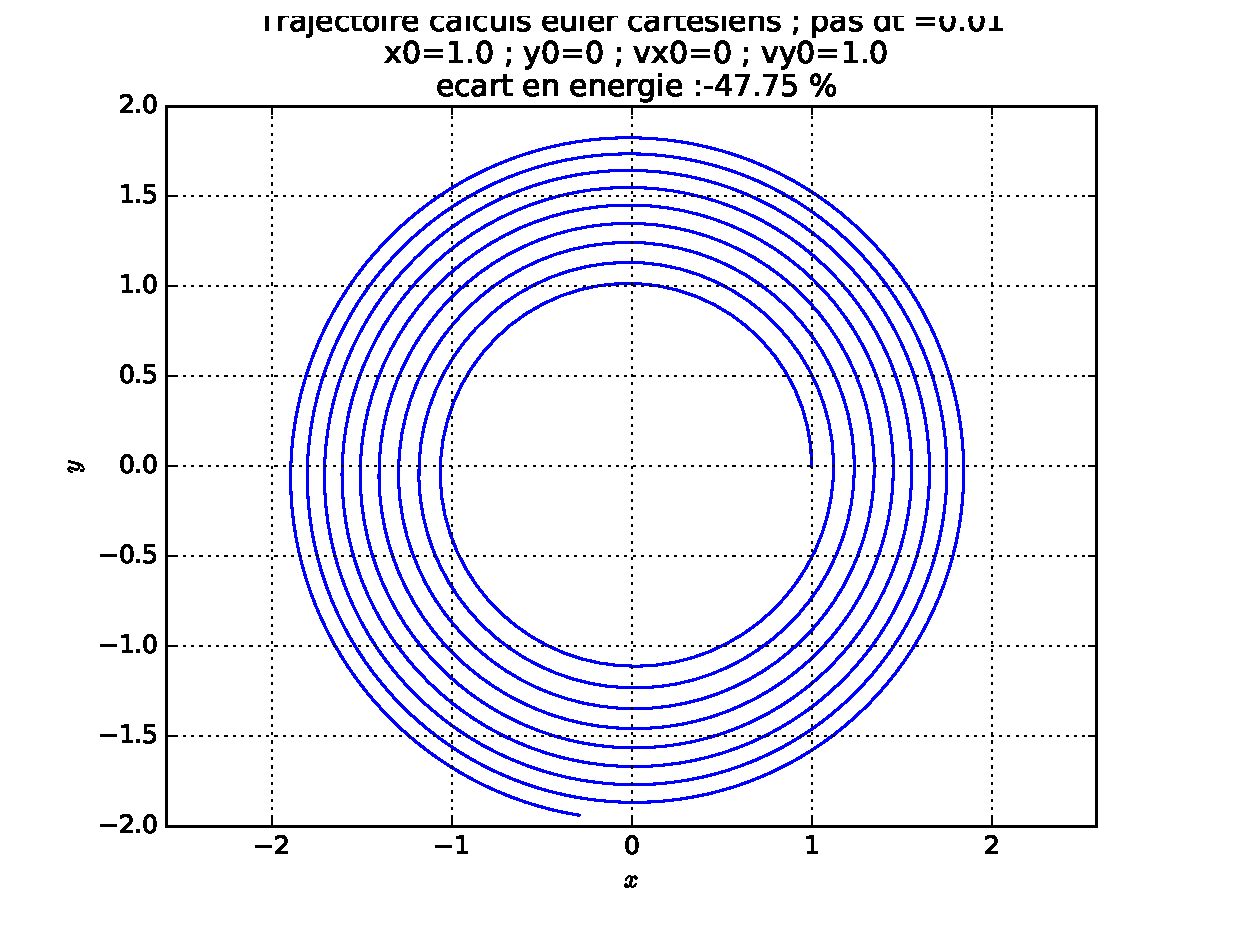
\includegraphics[width=7.5cm]{CartesienSimple}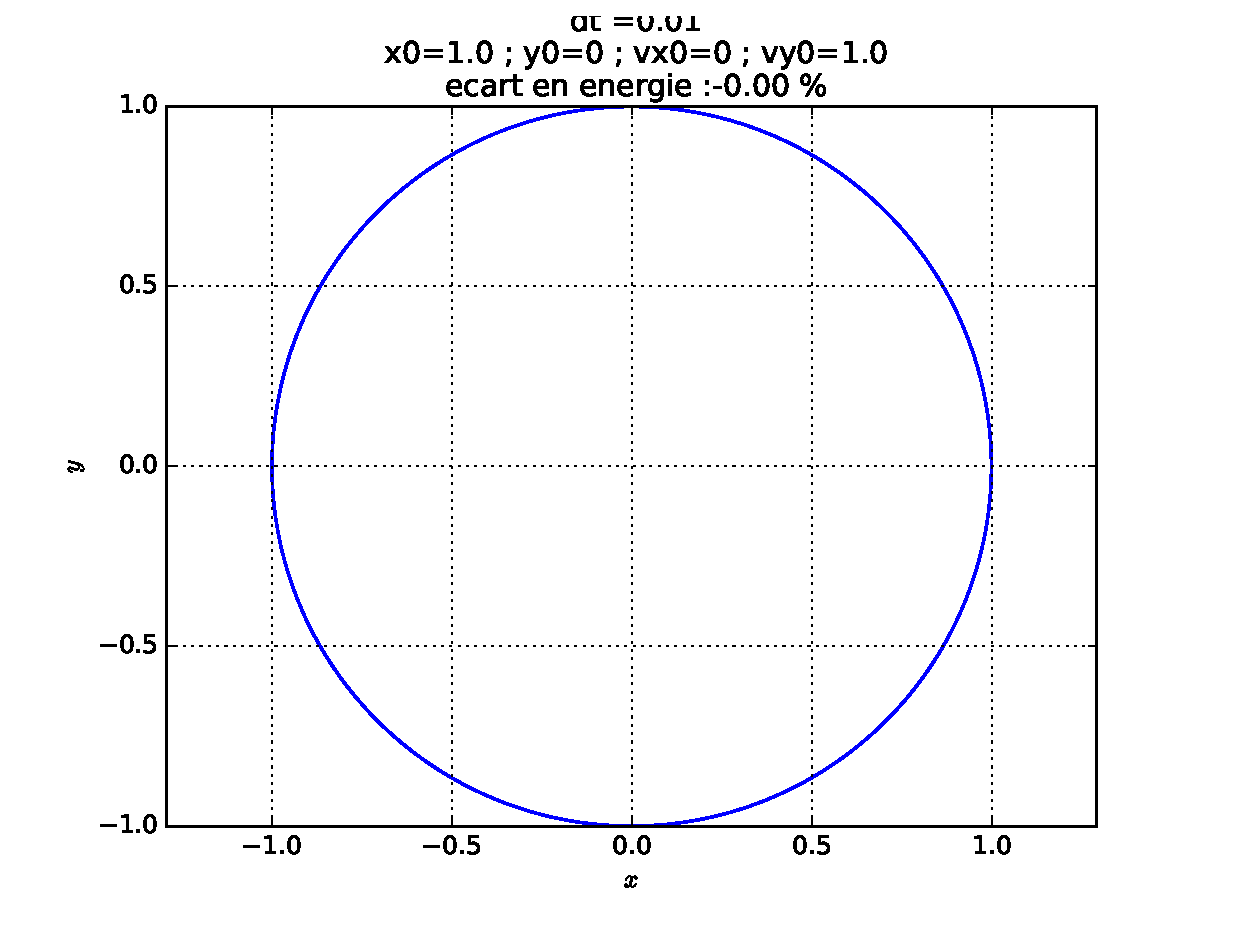
\includegraphics[width=7.5cm]{PolaireSimple1}%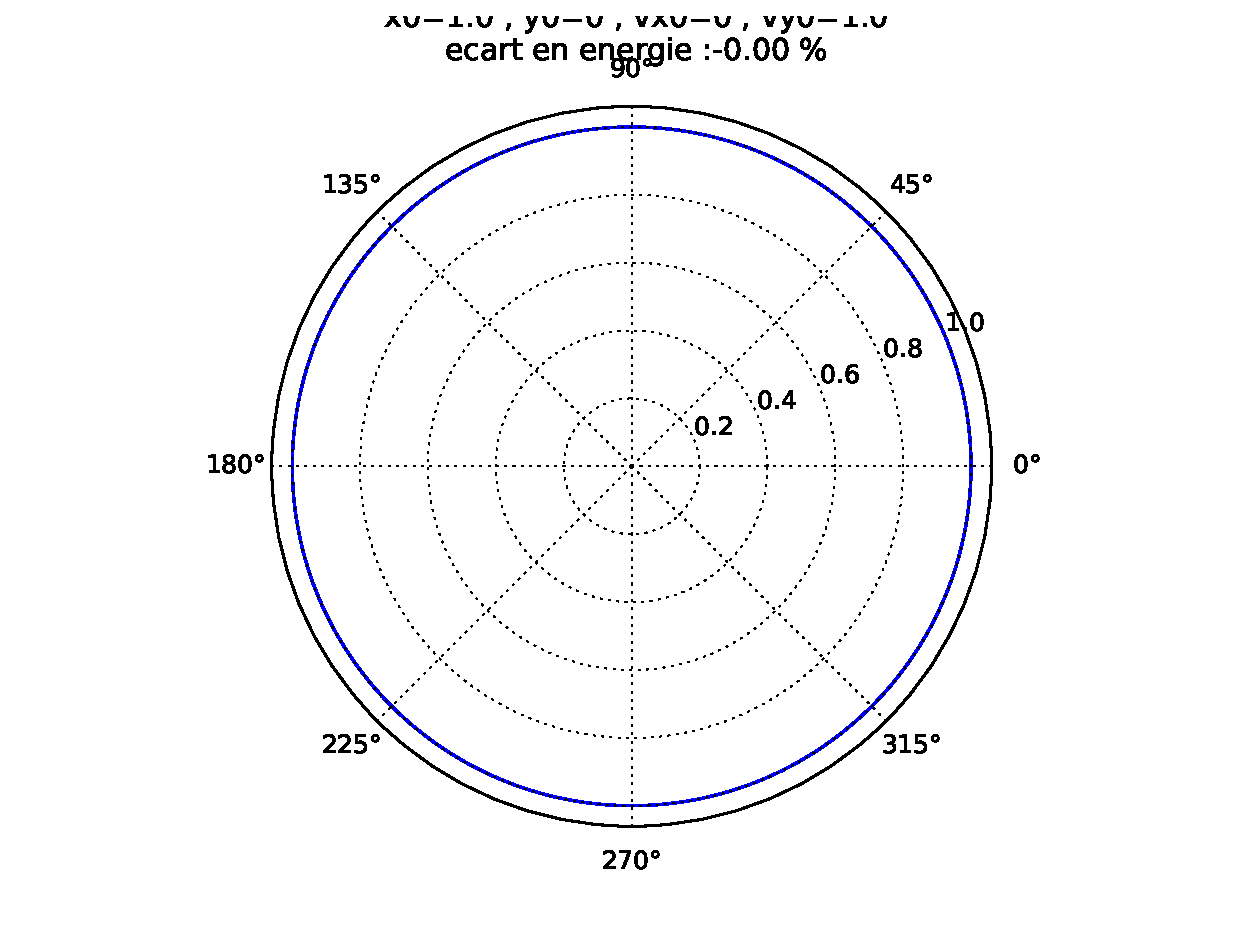
\includegraphics[width=5cm]{PolaireSimple2}
 \caption{Conditions initiales : $x0=1$, $y0=0$, $vx0=0$ $vy0=1$ ; pas d'intégration $dt = 0,01$. Figure de gauche : calculs en coordonnées cartésiennes. Figure de droite : calculs en coordonnées polaires. La trajectoire est censée être circulaire. On constate qu'en coordonnées polaires l'intégration est plus précise qu'en coordonnées cartésiennes.}
\end{figure}

\newpage
\section{Intégration par la méthode Leap-frog}

La version « saute-mouton » de l’algorithme d’Euler a plusieurs avantages sur sa version simple : meilleure conservation de l’énergie et invariance par renversement du temps en sont deux facettes. Pour limiter les complications, on se contentera de l’implémenter en coordonnées cartésiennes, mais avec des conditions initiales arbitraires en $x$ et en $y$ pour pouvoir vérifier le caractère invariant par retournement temporel. La méthode d’Euler précédente (à une seule variable) aurait pu s’écrire comme une suite de valeurs telles que :

\begin{center}$x_{n+1} = x_n + v_n\,\ud t \quad \textrm{et} \quad v_{n+1} = v_n + a_n\,\ud t$\end{center}

où l’accélération à l’étape $n$ ne dépend que de $x_n$ . En d’autres termes, les nouvelles valeurs des fonctions $x$ et $v$ sont calculées entièrement à partir des anciennes valeurs. Avec la méthode « saute-mouton », vitesse et position ne sont plus évaluées aux mêmes instants, la vitesse étant calculée pour des pas « demi-entiers » de sorte que position et vitesse puissent jouer à « saute-mouton » à tour de rôle l’un par-dessus l’autre :

\begin{center}$x_{n+1} = x_n + v_{n+\frac{1}{2}}\,\ud t \quad \textrm{et} \quad v_{n+\frac{1}{2}} = v_{n-\frac{1}{2}} + a_n\,\ud t$\end{center}

L’écriture semble bizarrement équivalente à la précédente mais, sous réserve d'une initialisation correcte, on peut montrer que la méthode a une précision quadratique\footnote{C'est-à-dire proportionnelle à $(\ud t)^2$. Voir Annexes.}, contrairement à la méthode d'Euler dont la précision est linéaire\footnote{C'est-à-dire proportionnelle à $\ud t$.}. La méthode d'initialisation pertinente est la suivante : pour un couple $(x_0,\, v_0)$ de conditions initiales, on initialise bien $x$ à $x_0$ , mais pour la vitesse, on initialise un demi pas plus tard : $v_{\frac{1}{2}} = v_0 + a_0\,\frac{\ud t}{2}$.

Vous pouvez à présent écrire la fonction \verb|leapfrog(position,vitesse,dt)|, où \verb|position| et \verb|vitesse| sont maintenant des doublets pour la position initiale \verb|(x0,y0)| et la vitesse initiale \verb|(vx0,vy0)|, et la comparer à \verb|euler(position,vitesse,dt)|, notamment au niveau de la conservation de l’énergie et de la réversibilité par renversement du temps (en d’autres termes, si on donne le point d’arrivée en \verb|t = 10| pour les deux procédures et que l’on inverse le signe des vitesses, la particule se retrouve-t-elle à \verb|t = 20| à l’endroit où elle se trouvait à \verb|t = 0| ?).

Une fois l'algorithme implanté en python, modifier les conditions initiales ($x_0$, $y_0$, $v_{x0}$ et $v_{y0}$), $dt$, $t_f$ pour voir leurs effets sur la précision de calcul et sur la trajectoire calculée.

\vspace{1cm}

\begin{figure}[htp]
 \centering
 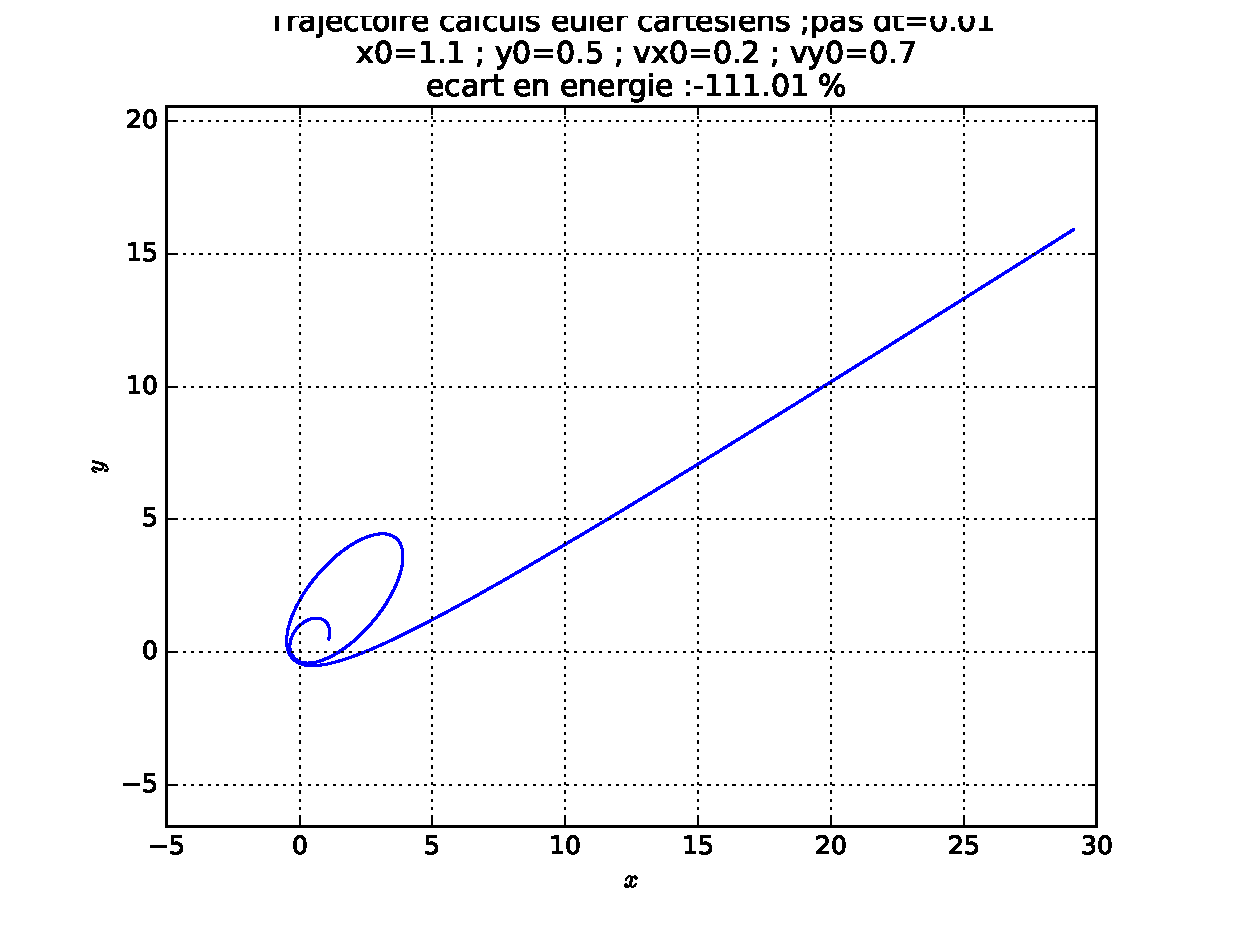
\includegraphics[width=5cm]{CartesienComplexe}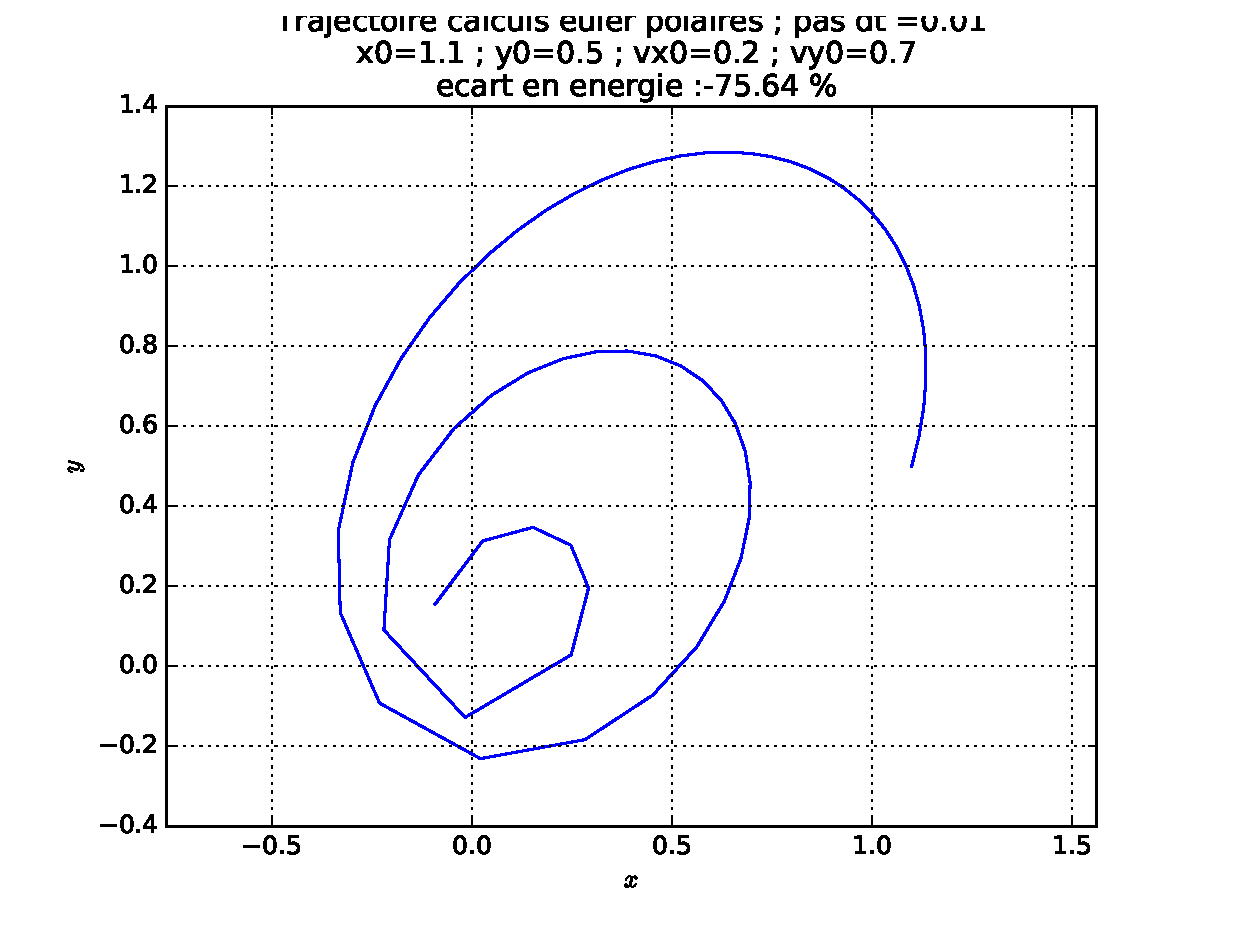
\includegraphics[width=5cm]{PolaireComplexe}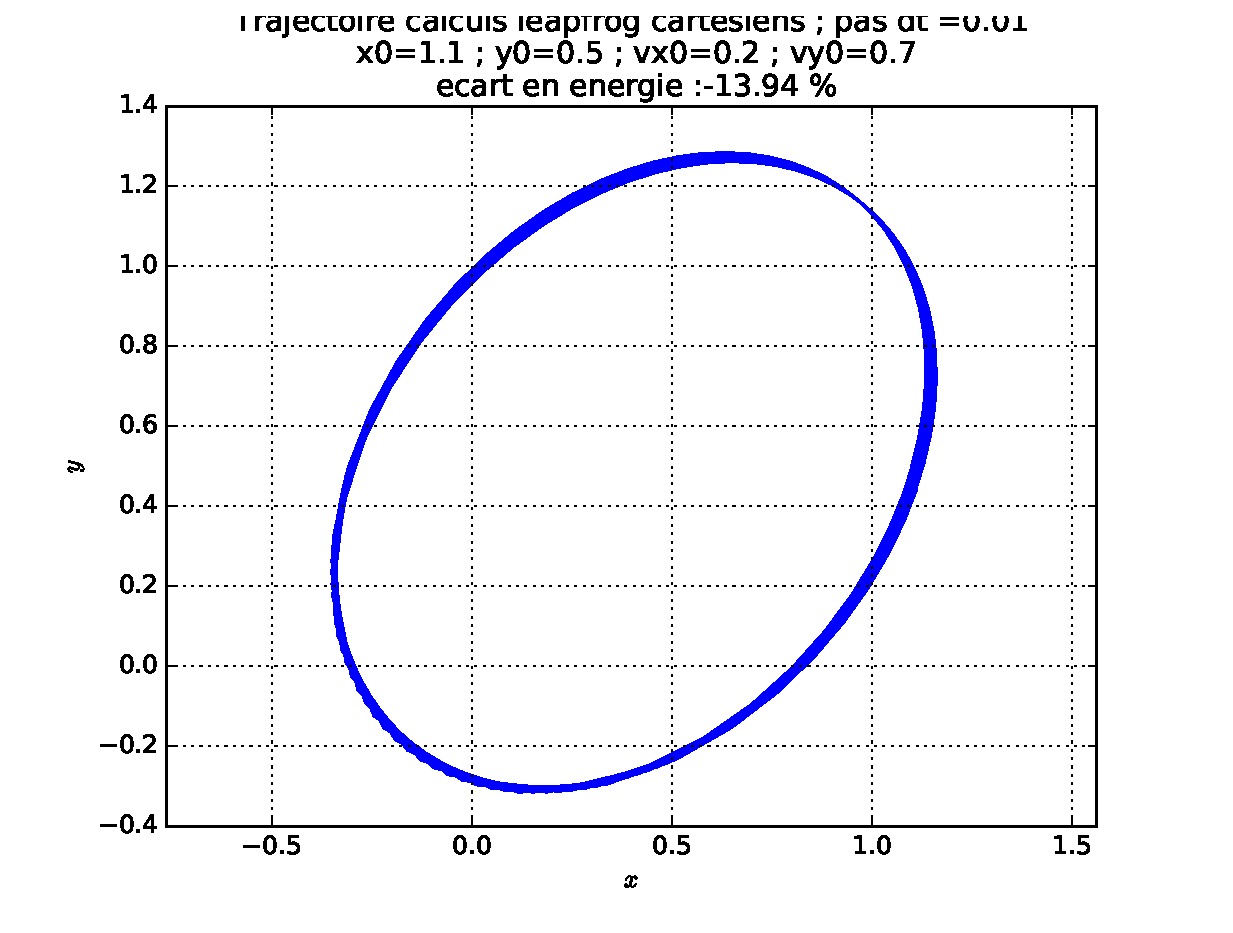
\includegraphics[width=5cm]{LeapFrogComplexe}
 \caption{Conditions initiales : $x0 = 1.1$, $y0= 0.5$ , $vx0 = 0.2$, $vy0 = 0.7$ ; pas d'intégration $dt = 0,01$. Figure de gauche : calculs en coordonnées cartésiennes. Figure du milieu : calculs en coordonnées polaires. Figure de droite : calculs en coordonnées cartésiennes avec la méthode Leap-frog. La trajectoire est censée être elliptique. On constate que, même en coordonnées cartésiennes, la méthode Leap-frog est la plus précise.}
\end{figure}

\newpage
\section*{Annexes}
\subsection*{Relations de passage de cartésiennes à polaires}

Dans un cas général, on a :
\begin{eqnarray*}
 \dot{r} &=& \frac{\dot{x}x}{\sqrt{x^2+y^2}} + \frac{\dot{y}y}{\sqrt{x^2+y^2}}\\
 \dot{\theta} &=& \frac{1}{\sqrt{x^2+y^2}}\,\left(\frac{-\dot{x}y}{\sqrt{x^2+y^2}} + \frac{\dot{y}x}{\sqrt{x^2+y^2}}\right)
\end{eqnarray*}


\subsection*{Précision de la méthode Leap-frog}
Dans la méthode Leap-frog, on itère par pas demi entier :
\begin{eqnarray}
x_{n+\frac{1}{2}} &=& x_n + \frac{1}{2}\,v_{n}\,\ud t\\
v_{n+1} &=& v_{n} + a_{n+\frac{1}{2}}\,\ud t\\
x_{n+1} &=& x_{n+\frac{1}{2}} + \frac{1}{2}\,v_{n+1}\,\ud t 
\end{eqnarray}

Si on injecte l'équation (1) dans l'équation (3), on obtient :
$$x_{n+1} = x_n + v_n\,\ud t + \frac{1}{2}\,a_{n+\frac{1}{2}}\,(\ud t)^2$$

La précision de l'algorithme semble donc bien quadratique. Néanmoins, la précision théorique de la méthode d'intégration est limitée par l'étape qui a la précision la plus faible. Si on n'y prend pas garde, c'est l'étape d'initialisation qui est le « maillon faible » de l'algorithme. En effet, la toute première demi-étape de mise à jour de la position (de 0 à $\frac{1}{2}$) : $$x_{\frac{1}{2}} = x_0 + \frac{1}{2}\,v_{0}\,\ud t$$ 

est de précision linéaire et donc malheureusement tout l'algorithme. On remédie à ce problème en utilisant, \textit{pour la toute première demi-étape uniquement}, la mise à jour suivante : 
$$x_{\frac{1}{2}} = x_0 + \frac{1}{2}\,v_{\frac{1}{2}}\,\ud t$$ 
avec 
$$v_{\frac{1}{2}} = v_0 + a_0\,\frac{\ud t}{2}$$
ce qui mène à 
$$x_{\frac{1}{2}} = x_0 + \frac{1}{2}\,v_{0}\,\ud t + \frac{1}{4}\,a_0\,(\ud t)^2$$ 

Ce qui prouve la précision quadratique de la première étape. Pour toutes les étapes ultérieures, on utilise les équations (1), (2) et (3) de l'algorithme Leap-frog qui sont équivalentes aux équations $x_{n+1} = x_n + v_{n+\frac{1}{2}}\,\ud t \quad \textrm{et} \quad v_{n+\frac{1}{2}} = v_{n-\frac{1}{2}} + a_n\,\ud t$ utilisées dans l'énoncé.

\end{document}
